%!TEX TS-program = xelatex
\documentclass[12pt, a4paper]{article}

%%%%%%%%%%%%%%%%%%%%%%%% Шрифты %%%%%%%%%%%%%%%%%%%%%%%%%%%%%%%%%
\usepackage{fontspec}         % пакет для подгрузки шрифтов
\setmainfont{MankSans}   % задаёт основной шрифт документа

%%%%%%%%%% Графика и рисование %%%%%%%%%%
\usepackage{tikz, pgfplots}  % язык для рисования графики из latex'a

\usepackage[paper=a4paper,top=5mm, bottom=5mm,left=15mm,right=15mm,includefoot,includehead]{geometry}


\usepackage{eso-pic}
\newcommand\Background{%
\parbox[b][\paperheight]{\paperwidth}{%
\vfill
\centering
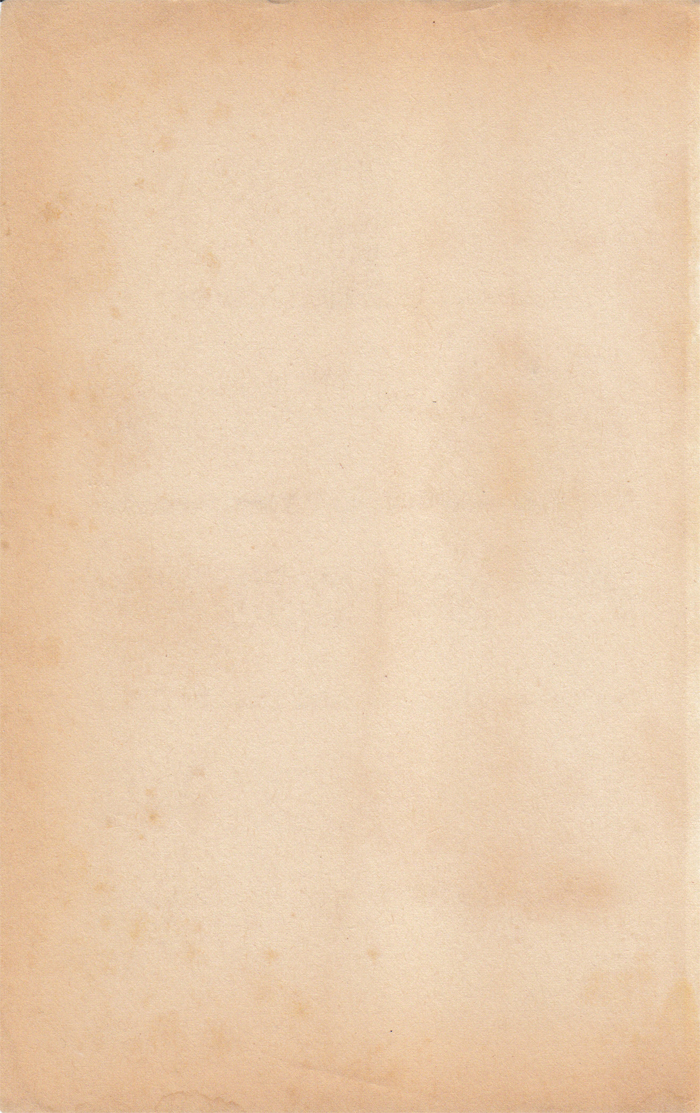
\includegraphics[ width=\paperwidth, height=\paperheight]{Vintage.jpg}%
\vfill
}}

\usepackage{pgf}
\usetikzlibrary{arrows}
\usetikzlibrary{calc}


\begin{document} % конец преамбулы, начало документа

\thispagestyle{empty}
\AddToShipoutPicture*{\Background}

\begin{tikzpicture}[overlay,remember picture]
    \draw [line width=1pt,rounded corners=1pt,
        ]
        ($ (current page.north west) + (1cm,-1cm) $)
        rectangle
        ($ (current page.south east) + (-1cm,1cm) $);
        
    \draw [line width=1pt,rounded corners=1pt]
        ($ (current page.north west) + (1.2cm,-1.2cm) $)
        rectangle
        ($ (current page.south east) + (-1.2cm,1.2cm) $);
\end{tikzpicture}


\center{\fontsize{48}{1.33}\selectfont \fontspec{Ruritania}{Contract}}

\vspace{30ex}

\center{\fontsize{24}{1.33}\selectfont I agree to take the job.}

\vspace{8ex}

\begin{tikzpicture}[line cap=round,line join=round,>=triangle 45,x=1.0cm,y=1.0cm]
\clip(-10.021978415601811,-3.8905958144160557) rectangle (10.238112192747513,6.362771780418124);
\draw [line width=0.4pt,dash pattern=on 2pt off 2pt] (4.62,2.18)--  (4.62,2.18)-- (4.56,2.08)-- (4.52,2.02)-- (4.48,1.96)-- (4.46,1.9)-- (4.44,1.82)-- (4.42,1.76)-- (4.4,1.7)-- (4.38,1.62)-- (4.34,1.56)-- (4.3,1.5)-- (4.24,1.46)-- (4.2,1.4)-- (4.18,1.34)-- (4.18,1.26)-- (4.18,1.14)-- (4.18,1.04)-- (4.2,0.96)-- (4.24,0.9)-- (4.3,0.86)-- (4.36,0.78)-- (4.42,0.76)-- (4.48,0.74)-- (4.56,0.7)-- (4.64,0.68)-- (4.72,0.68)-- (4.8,0.7)-- (4.88,0.76)-- (4.96,0.8)-- (5.02,0.86)-- (5.04,0.92)-- (5.06,1.)-- (5.08,1.12)-- (5.1,1.24)-- (5.1,1.32)-- (5.08,1.38)-- (5.06,1.44)-- (5.04,1.5)-- (5.04,1.58)-- (5.04,1.66)-- (5.02,1.74)-- (5.02,1.86)-- (5.04,1.92)-- (5.08,1.98)-- (5.08,2.06)-- (5.06,2.12)-- (5.,2.18)-- (4.92,2.22)-- (4.86,2.26)-- (4.8,2.28)-- (4.72,2.28)-- (4.66,2.26)-- (4.62,2.2)-- (4.6,2.14)-- (4.64,2.08);
\draw [line width=0.4pt,dash pattern=on 2pt off 2pt] (6.08,0.06)--  (6.08,0.06)-- (6.02,0.1)-- (5.94,0.14)-- (5.86,0.14)-- (5.76,0.14)-- (5.7,0.12)-- (5.64,0.1)-- (5.58,0.06)-- (5.48,0.04)-- (5.42,0.02)-- (5.36,0.)-- (5.3,-0.02)-- (5.24,-0.08)-- (5.18,-0.12)-- (5.12,-0.16)-- (5.06,-0.2)-- (5.,-0.22)-- (4.98,-0.28)-- (4.96,-0.34)-- (4.98,-0.44)-- (5.,-0.54)-- (5.02,-0.62)-- (5.04,-0.68)-- (5.06,-0.76)-- (5.08,-0.86)-- (5.1,-0.94)-- (5.14,-1.)-- (5.2,-1.08)-- (5.26,-1.14)-- (5.32,-1.18)-- (5.38,-1.2)-- (5.44,-1.22)-- (5.54,-1.24)-- (5.62,-1.26)-- (5.7,-1.3)-- (5.76,-1.32)-- (5.8,-1.38)-- (5.84,-1.44)-- (5.9,-1.48)-- (6.,-1.48)-- (6.12,-1.46)-- (6.2,-1.44)-- (6.26,-1.38)-- (6.34,-1.3)-- (6.38,-1.24)-- (6.42,-1.18)-- (6.46,-1.12)-- (6.48,-1.06)-- (6.5,-1.)-- (6.5,-0.92)-- (6.5,-0.84)-- (6.46,-0.78)-- (6.4,-0.76)-- (6.32,-0.72)-- (6.26,-0.68)-- (6.22,-0.62)-- (6.18,-0.56)-- (6.12,-0.52)-- (6.08,-0.46)-- (6.04,-0.4)-- (6.02,-0.34)-- (6.06,-0.26)-- (6.12,-0.2)-- (6.18,-0.16)-- (6.22,-0.1)-- (6.22,-0.02)-- (6.16,0.)-- (6.1,0.04)-- (6.04,0.06);
\draw [line width=0.4pt,dash pattern=on 2pt off 2pt] (4.3,0.34)-- (4.3,0.34)-- (4.24,0.38)-- (4.18,0.4)-- (4.1,0.4)-- (4.04,0.42)-- (3.98,0.44)-- (3.88,0.44)-- (3.8,0.44)-- (3.76,0.38)-- (3.76,0.3)-- (3.76,0.22)-- (3.74,0.16)-- (3.74,0.08)-- (3.72,0.02)-- (3.72,-0.06)-- (3.74,-0.12)-- (3.82,-0.16)-- (3.9,-0.18)-- (3.98,-0.2)-- (4.04,-0.24)-- (4.1,-0.28)-- (4.16,-0.34)-- (4.2,-0.4)-- (4.26,-0.44)-- (4.28,-0.5)-- (4.36,-0.48)-- (4.4,-0.42)-- (4.42,-0.34)-- (4.44,-0.28)-- (4.46,-0.22)-- (4.48,-0.16)-- (4.52,-0.1)-- (4.5,-0.04)-- (4.44,-0.02)-- (4.38,0.02)-- (4.38,0.1)-- (4.32,0.16)-- (4.3,0.22)-- (4.3,0.3)-- (4.28,0.36);
\draw [line width=0.4pt,dash pattern=on 2pt off 2pt] (5.86,0.8)-- (5.86,0.8)-- (5.8,0.78)-- (5.78,0.72)-- (5.74,0.66)-- (5.7,0.6)-- (5.68,0.54)-- (5.74,0.52)-- (5.8,0.5)-- (5.88,0.5)-- (5.96,0.5)-- (6.02,0.52)-- (6.08,0.54)-- (6.12,0.6)-- (6.12,0.68)-- (6.06,0.7)-- (6.,0.76)-- (5.94,0.78)-- (5.88,0.8)-- (5.82,0.76);
\draw [line width=0.4pt,dash pattern=on 2pt off 2pt] (5.66,1.54)--  (5.66,1.54)-- (5.64,1.6)-- (5.62,1.66)-- (5.62,1.74)-- (5.68,1.78)-- (5.76,1.78)-- (5.82,1.76)-- (5.82,1.68)-- (5.84,1.62)-- (5.84,1.54)-- (5.86,1.48)-- (5.92,1.44)-- (5.92,1.36)-- (5.9,1.3)-- (5.84,1.28)-- (5.76,1.28)-- (5.74,1.34)-- (5.72,1.4)-- (5.7,1.46)-- (5.64,1.48)-- (5.64,1.56);
\draw (2.6667958476046456,-1.88220422367534) node[anchor=north west] {\fontspec{MankSans}{Place for a drop of blood}};
\end{tikzpicture}

\vspace{6ex}

\color{darkgray}{\underline{\hspace{13cm}}}
\makebox[13em]{\hfill\footnotesize SIGNATURE \hfill}

\end{document}